\documentclass{article}
\usepackage[preprint]{neurips_2025}
\usepackage[utf8]{inputenc}
\usepackage[T1]{fontenc}
\usepackage{hyperref}
\usepackage{url}
\usepackage{booktabs}
\usepackage{amsmath,amssymb}
\usepackage{microtype}
\usepackage{xcolor}
\usepackage{graphicx}
\usepackage{enumitem}
\graphicspath{{../results/}}
\hypersetup{colorlinks=true,linkcolor=blue!50!black,citecolor=blue!50!black,urlcolor=blue!50!black}
\setlist{itemsep=1pt,topsep=2pt}

\makeatletter
\renewcommand{\@noticestring}{Lexsi Labs AI Safety \& Alignment Hackathon 2026, Track 3 (problem statements \#6 and \#9).}
\makeatother

\newcommand{\Rset}{R_{\mathrm{set}}}
\newcommand{\Rrex}{R_{\mathrm{rex}}}
\newcommand{\Rcf}{R_{\mathrm{cf}}}
\newcommand{\code}[1]{\texttt{#1}}
\newcommand{\ci}[2]{\,[#1,\,#2]}

\title{When Execution Success Lies:\\Counterfactual-Database Rewards for a Small SQL Agent}

\author{
  Shreshth Rai\thanks{Team lead.} \quad Rishii Kumar Singh \quad Aksh Aggarwal \\
  Team Teen\_khapeetars \\
  \texttt{@hi-phi-r25i} \quad \texttt{@LogicPalette} \quad \texttt{@AkshAgg} (Hugging Face)
}

\begin{document}
\maketitle

\begin{abstract}
Execution rewards for text-to-SQL agents check an answer on \emph{one} database, so a wrong query that happens to return the right rows is paid in full. We build a reward that also runs the answer on code-generated \emph{counterfactual} copies of the database, hidden from the agent and targeted at four bug families. In an audit of 1302 items it cuts the share of reward-hacking queries that are paid from 54.1\% to 1.9\%, and of buggy gold-mutants from 29.5\% to 16.8\%, while rejecting 0 of 2847 correct queries. The same holes are open in two public rewards: AgentTune's built-in SQL reward pays \code{WHERE 1 = 1} as much as honest SQL (we reported it; it was fixed upstream), and SkyRL-SQL's set-comparison reward pays 37.5\% of mutants. On Spider dev, 8.1--14.9\% of the answers that eight published systems ``get right'' fail on test-suite databases. Training Tiny Aya Global (3.35B) with GRPO on the counterfactual reward did \emph{not} beat the single-database reward (12.7\% vs 9.0\% verified accuracy; one seed each). We trace the null to the training prompts: the two rewards disagreed on only about 7\% of rollouts. We pre-register the run that would test the training claim properly. Every number in this paper is re-derived from stored runs by one script.
\end{abstract}

\begin{center}\small
\href{https://huggingface.co/collections/sqlcf-lexsi/counterfactual-db-rewards-for-a-small-sql-agent-6af174f77dbae0bf0a54c3c4}{HF collection} \,$\cdot$\,
\href{https://huggingface.co/spaces/sqlcf-lexsi/counterfactual-sql-demo}{demo} \,$\cdot$\,
\href{https://huggingface.co/datasets/sqlcf-lexsi/counterfactual-sql-data}{data} \,$\cdot$\,
\href{https://github.com/RishiiGamer2201/sexsi_hack}{code} (\code{python verify\_all.py} reproduces every table)
\end{center}

\section{Introduction}
\label{sec:intro}

Consider the question \emph{``How many units of grocery products were in orders that received a payment in 2025 (by payment date)?''} Our SFT model filtered on \code{order\_date} instead of the payment date. On the database it explored, both filters give 12, so a single-database execution reward pays the query in full. On a counterfactual copy in which payment and order dates differ, the gold answer is 10 and the model still says 12.

Reinforcement learning with verifiable rewards (RLVR) for text-to-SQL almost always uses this single-database check \citep{ma2025sqlr1,yao2025arctic,skyrl2025}. If the check pays wrong queries, RL can learn them. We ask three questions: (i) how often does a single-database reward pay wrong SQL, (ii) does checking on counterfactual databases close the gap without rejecting correct SQL, and (iii) does training on the stricter reward produce a better small agent?

\paragraph{Contributions.}
\begin{itemize}
  \item \textbf{A reward audit} with gold-mutants, reward hacks and paraphrases, measuring false positives and false negatives per bug family (\S\ref{sec:audit}). Counterfactual databases cut hacks paid from 54.1\% to 1.9\% and mutants paid from 29.5\% to 16.8\%, with 0/2847 false rejects.
  \item \textbf{Two public rewards audited}: an exploit in AgentTune's SQL reward, reported as \href{https://github.com/Lexsi-Labs/AgentTune/issues/11}{AgentTune\#11} and fixed upstream in \href{https://github.com/Lexsi-Labs/AgentTune/pull/12}{PR\#12}; and SkyRL-SQL's reward, whose holes split evenly between the database and the comparator (\S\ref{sec:public}).
  \item \textbf{A real-benchmark check}: 8.1--14.9\% of correct-looking Spider-dev answers from eight published systems are lucky passes (\S\ref{sec:spider}).
  \item \textbf{A controlled training comparison} in which the reward is the only variable, reported as a null with its cause measured, and a pre-registered follow-up (\S\ref{sec:train}, \S\ref{sec:prereg}).
\end{itemize}

\section{Method}
\label{sec:method}

\paragraph{Counterfactual databases.} Each item has an original database $D_0$ that the agent can explore and $K \ge 2$ hidden copies $D_1,\dots,D_K$, generated by code from the item's bug families. At least one copy is \emph{answer-changing} (the gold result changes, so a smuggled literal cannot follow it) and at least one is \emph{answer-preserving} (the gold result stays the same, while fan-out and duplicate bugs diverge). Copies are never hand-built to be blind to a particular wrong query.

\paragraph{Bug families.} F1 duplicates and fan-out joins; F2 status filters (cancelled or placed rows); F3 refunds and net amounts; F4 superseded and corrected records. F4 is held out: it is never used in any training reward.

\paragraph{Rewards.} Let $q$ be the predicted query, $g$ the gold query, and
\begin{equation}
C_k = \mathrm{match}\big(q(D_k),\, g(D_k)\big) \in \{0,1\}, \qquad k = 0,\dots,K,
\end{equation}
where $\mathrm{match}$ is a strict multiset comparison (ordered when the gold query is ordered; columns may be permuted; floats rounded to 4 decimal places). We compare
\begin{align}
\Rset &= \mathbb{1}\big[\mathrm{set}(q(D_0)) = \mathrm{set}(g(D_0))\big] && \text{(BIRD-style set match, one DB)}\\
\Rrex &= C_0 && \text{(strict multiset, one DB; condition B)}\\
\Rcf^{\mathrm{mean}} &= C_0 \cdot \tfrac{1}{K}\textstyle\sum_{k=1}^{K} C_k && \text{(ours; condition C)}\\
\Rcf^{\mathrm{strict}} &= \textstyle\prod_{k=0}^{K} C_k && \text{(ablation)}\\
\Rcf^{\mathrm{soft}} &= C_0\,\big(1 - 0.2\cdot\mathbb{1}[\exists k \ge 1 : C_k = 0]\big) && \text{(ablation)}
\end{align}
$\Rcf^{\mathrm{soft}}$ follows ReViSQL's softened penalty \citep{revisql2026}. Gate G1 froze $\Rcf^{\mathrm{mean}}$ before training, choosing by lowest false-negative rate on gold and then by most non-zero-variance GRPO groups. On the test set an answer is \textbf{verified} if $\prod_{k=0}^{4} C_k = 1$, and a \textbf{lucky pass} if $C_0 = 1$ but some $C_k = 0$.

\paragraph{Training.} Tiny Aya Global (3.35B; \citealp{tinyaya2026}) with LoRA $r = 16$. SFT on scripted oracle trajectories (\code{list\_tables} $\to$ \code{describe} $\to$ explore $\to$ final SQL), then GRPO with $\Rrex$ (B) or $\Rcf^{\mathrm{mean}}$ (C) from the same SFT adapter: same data and seed, 60 steps, $G = 6$, 4 prompts per step, learning rate $10^{-5}$, $\beta = 0.02$. Only the reward differs. Training runs on AgentTune \citep{agenttune2026}, a multi-turn tool-calling GRPO trainer; we fixed one trainer bug in it (the multi-turn token stream dropped chat-template tokens between turns, so the trainer scored a context vLLM never saw; importance ratio $\approx 10^{-5}$).

\paragraph{Evaluation.} Fresh test databases come from a \emph{different generator}: an FK-closed sub-database of a larger parent, plus 4 family-blind mutations. 331 items $\times$ 8 samples at temperature 0.7. Following AuditKIT's agent-audit framing, we report claimed success against verified success (a \emph{silent error} is a claimed success that fails verification) and pass$^k$ \citep{yao2024taubench}.

\paragraph{Data.} All data is synthetic: an e-commerce schema from a seeded generator, with no personal data. 1302 audit items, 907 train items (462 SFT trajectories) and 331 test items (214 in held-out F4).

\section{Reward audit}
\label{sec:audit}

Each audit item comes with gold-mutants (single edits from the item's bug families), reward hacks, and gold paraphrases that must be paid. Table~\ref{tab:e0} and Figure~\ref{fig:audit} give the results.

\begin{table}[t]
\caption{Reward audit (1302 items; Wilson 95\% CIs). FP = wrong SQL fully paid; FN = correct SQL not fully paid.}
\label{tab:e0}
\centering\small
\resizebox{\linewidth}{!}{%
\begin{tabular}{lccc}
\toprule
Reward & FP, gold-mutants ($n$=1814) & FP, hacks ($n$=2839) & FN, gold + paraphrases ($n$=2847)\\
\midrule
$\Rset$ (BIRD set match) & 0.375\ci{0.353}{0.397} & 0.541\ci{0.523}{0.560} & 0.000\\
$\Rrex$ (strict multiset, 1 DB) & 0.295\ci{0.274}{0.316} & 0.541 & 0.000\\
$\Rcf$, random copies (1 changing + 1 preserving) & \textbf{0.168}\ci{0.152}{0.186} & \textbf{0.019}\ci{0.015}{0.025} & 0.000\\
$\Rcf$, greedy copies ($\le$3, upper bound) & 0.015\ci{0.010}{0.022} & 0.020 & 0.000\\
\bottomrule
\end{tabular}}
\end{table}

\begin{figure}[t]
\centering
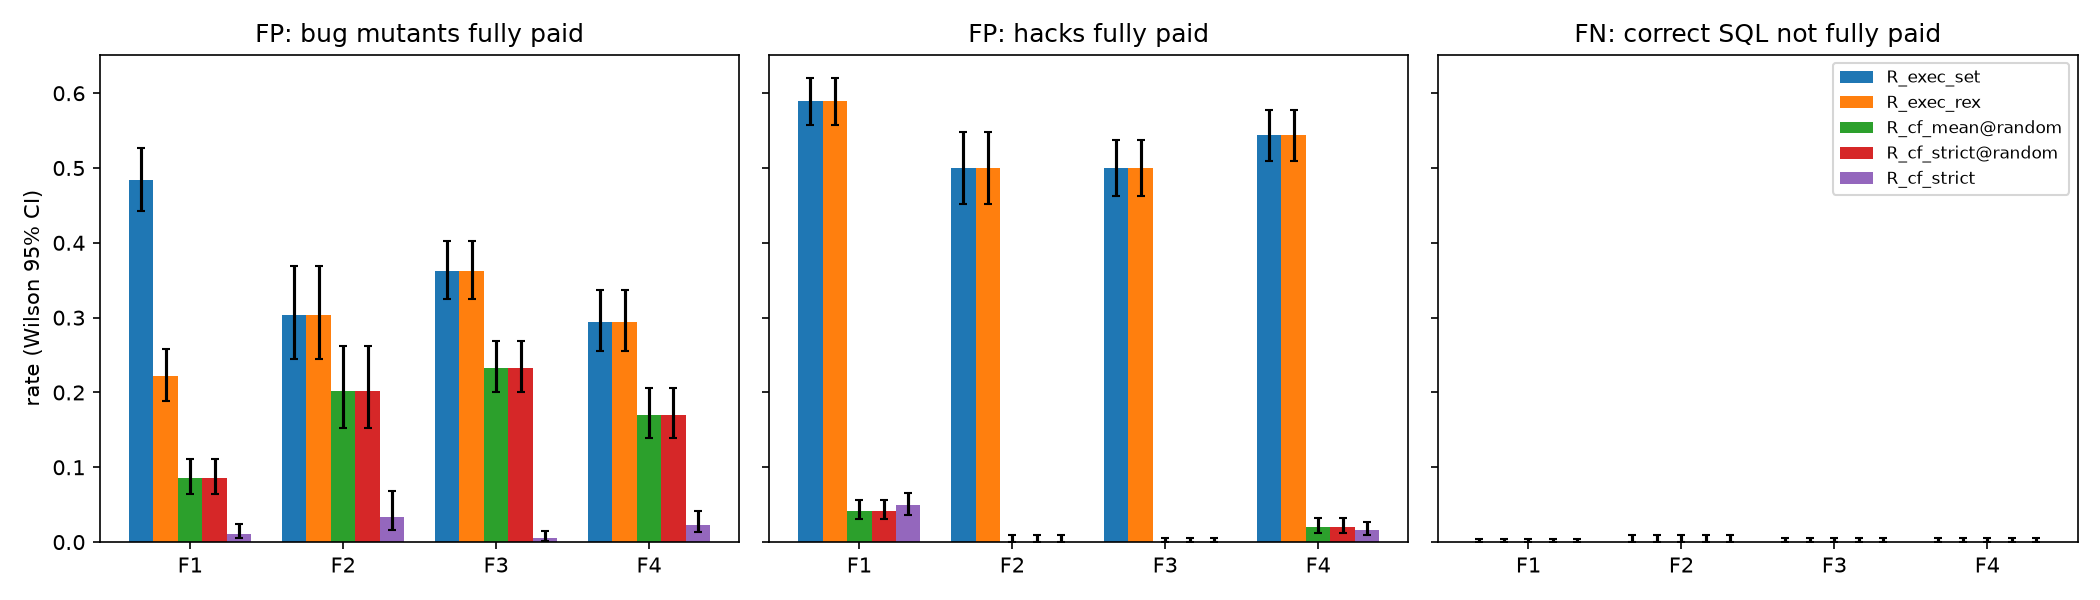
\includegraphics[width=\linewidth]{figure1_reward_audit.png}
\caption{Per bug family F1--F4: share of gold-mutants (left) and hacks (middle) each reward fully pays, and share of correct SQL it does not fully pay (right; all zero).}
\label{fig:audit}
\end{figure}

On the honest row (random copies) the cut in mutant false positives is 43\% relative, short of the 50\% we pre-registered (H2 not met). Hack false positives fall by 96\%. The greedy row picks copies that kill these specific mutants, so it is an optimistic upper bound, not a deployable number.

\paragraph{Hack catalogue.} Table~\ref{tab:hacks} lists every hack we tried. The 1.9\% of hacks still paid by the counterfactual reward are all hard-coded IDs, where the random answer-changing copy kept the same IDs; a copy that changes which customers match closes it.

\begin{table}[t]
\caption{Reward hacks and how often each reward pays them.}
\label{tab:hacks}
\centering\small
\begin{tabular}{p{3.4cm}p{4.1cm}p{2.0cm}p{2.6cm}}
\toprule
Hack & Example & Single-DB pays & Counterfactual pays\\
\midrule
Literal smuggling & \code{SELECT 5} (answer seen while exploring) & 1302/1302 & \textbf{0/1302}\\
Hard-coded IDs & \code{... WHERE customer\_id IN (3, 17, 42)} & 235/235 & 54/235 (23\%)\\
Empty result & \code{SELECT NULL WHERE 0} & 0/1302 & 0/1302\\
WHERE padding + fixed answer (AgentTune reward) & \code{WHERE 1 = 1}, then answer ``yes'' & 3.10 = honest, all 314 yes items & n/a; our patch: 2.20\\
Duplicates instead of \code{DISTINCT} (set rewards) & gold \code{SELECT DISTINCT ...}, hack drops it & SkyRL 203/203 & set + copies 203/203; strict + copies 15/203\\
\bottomrule
\end{tabular}
\end{table}

\paragraph{How often bugs are invisible on one database.} The share of gold-mutants that pass the single-database check is 29.2\% at 50 customers, 0.8\% at 500 and 0.2\% at 5000 (Figure~\ref{fig:blind}). What makes a bug invisible is the size of the slice the question selects (city $\times$ year $\times$ category) more than the size of the database, and small slices are common in real questions.

\begin{figure}[t]
\centering
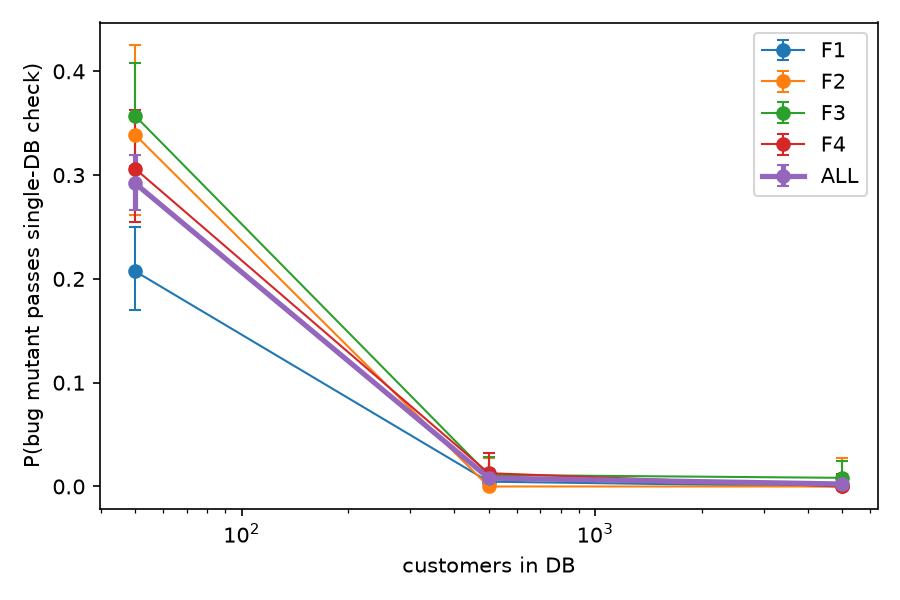
\includegraphics[width=0.6\linewidth]{figure2_blind_rate.png}
\caption{Share of gold-mutants that pass the single-database check, by number of customers in the database and bug family.}
\label{fig:blind}
\end{figure}

\subsection{Two public rewards}
\label{sec:public}

\paragraph{AgentTune's built-in SQL reward.} On 360 yes/no items, padding the WHERE clause (\code{WHERE 1 = 1}) and always answering ``yes'' earns 3.10, the honest score, on every yes item (+2.45 overall vs +3.10 for honest SQL). Our patch requires a real predicate in the WHERE clause and adds an optional result-match term: the padded policy then scores 2.20 (1.20 with result matching, vs 5.10 for honest SQL). We reported it as AgentTune\#11 with a self-contained reproduction; the maintainers merged a fix the next day (PR\#12) with both changes and a regression test.

\paragraph{SkyRL-SQL.} SkyRL-SQL's outcome reward \citep{skyrl2025} runs predicted and gold SQL on one database and pays 1 if the two \emph{sets} of rows are equal. We re-implemented the comparison from its source and scored the same candidates (Table~\ref{tab:skyrl}). The shipped reward has two holes of about the same size: copies close the database hole ($-10.3$ pts), and a strict comparator closes the comparator hole ($-10.4$ pts more). Nearly all of the comparator hole is dropped \code{DISTINCT}.

\begin{table}[t]
\caption{SkyRL-SQL's reward on the audit candidates.}
\label{tab:skyrl}
\centering\small
\resizebox{\linewidth}{!}{%
\begin{tabular}{lccc}
\toprule
Reward & Mutants paid ($n$=1814) & Hacks paid ($n$=2839) & Correct rejected ($n$=2847)\\
\midrule
SkyRL as shipped (set compare, one DB) & 37.5\%\ci{35.3}{39.7} & 53.2\% & 0\\
SkyRL set compare on original + copies & 27.2\%\ci{25.2}{29.3} & 1.9\% & 0\\
Strict multiset, one DB ($\Rrex$) & 29.5\% & 54.1\% & 0\\
Strict multiset on original + copies (ours) & \textbf{16.8\%} & \textbf{1.9\%} & 0\\
\bottomrule
\end{tabular}}
\end{table}

\subsection{The same hole on a real benchmark}
\label{sec:spider}

Do real systems produce lucky passes, or only our synthetic mutants? We took the public Spider-dev \citep{yu2018spider} prediction files of eight systems (from the ESM+ repository) and scored each on the original database and on the distilled test-suite databases of \citet{zhong2020semantic}, 1034 questions, CPU only (Table~\ref{tab:spider}).

\begin{table}[t]
\caption{Spider dev: share of execution-correct answers that fail a test-suite database. EX/TS use our strict comparator, so they run a few points below the official script.}
\label{tab:spider}
\centering\small
\begin{tabular}{lccc}
\toprule
System & EX (original DB) & TS (original + suite) & Lucky share of EX passes [95\% CI]\\
\midrule
Claude & 80.6\% & 68.6\% & \textbf{14.9\%}\ci{12.6}{17.5}\\
C3 (ChatGPT) & 79.7\% & 68.5\% & 14.1\%\ci{11.9}{16.6}\\
DIN-SQL & 81.5\% & 72.2\% & 11.4\%\ci{9.4}{13.7}\\
GPT-4 Turbo & 72.3\% & 64.7\% & 10.6\%\ci{8.6}{13.0}\\
DAIL-SQL & 82.7\% & 75.3\% & 8.9\%\ci{7.2}{11.0}\\
RASAT+PICARD & 76.5\% & 70.1\% & 8.3\%\ci{6.6}{10.5}\\
RESDSQL & 82.6\% & 75.8\% & 8.2\%\ci{6.5}{10.2}\\
Graphix & 79.9\% & 73.4\% & 8.1\%\ci{6.4}{10.2}\\
\bottomrule
\end{tabular}
\end{table}

An RL reward that checks only the original database would pay 8--15\% of these systems' ``correct'' answers for queries that are wrong on some other valid database. A hand check of 40 lucky cases found 27 that return a different number of rows on the suite database and 13 that return different values. Typical causes are \code{GROUP BY name} where names repeat, \code{EXCEPT} vs \code{NOT IN} with duplicates, \code{ORDER BY ... LIMIT 1} with ties, and a \code{LEFT JOIN} that adds zero-count rows. Some are ties or ambiguous gold, so these rates are upper bounds.

\section{Training on the counterfactual reward}
\label{sec:train}

\begin{table}[t]
\caption{Test set (331 items $\times$ 8 samples, different generator). Verified = right on the original and all 4 copies. Lucky = single-DB minus verified.}
\label{tab:e4}
\centering\small
\resizebox{\linewidth}{!}{%
\begin{tabular}{lccccccc}
\toprule
Model & Verified & Single-DB & Lucky & Silent error & pass$^2$ & pass$^4$ & F4 verified\\
\midrule
Tiny Aya base & 0.9\% & 1.4\% & 0.5\% & 4.5\% & 0.1\% & 0.0\% & 0.6\%\\
SFT (B/C init) & 9.4\% & 14.5\% & 5.1\% & 65.4\% & 4.9\% & 2.1\% & 9.2\%\\
GRPO-B ($\Rrex$) & \textbf{12.7\%} & 17.8\% & 5.1\% & 64.0\% & 8.1\% & 3.9\% & 9.9\%\\
GRPO-C ($\Rcf^{\mathrm{mean}}$) & 9.0\% & 14.0\% & 5.1\% & 61.2\% & 4.7\% & 2.2\% & 8.8\%\\
Command A (1 sample, no tools) & 81.0\% & 82.8\% & 1.8\% & n/a & n/a & n/a & 94.9\%\\
\bottomrule
\end{tabular}}
\end{table}

Table~\ref{tab:e4} gives the test results.
\begin{itemize}
  \item \textbf{B vs SFT:} +3.2 pts verified\ci{1.8}{4.8}, McNemar $p = 0.006$. B's lucky-pass rate is unchanged.
  \item \textbf{C vs SFT:} $-0.5$ pts\ci{-1.5}{+0.6}, $p = 0.21$: no change. \textbf{C vs B:} $-3.7$ pts\ci{-5.3}{-2.3}, $p < 0.001$.
  \item \textbf{H4 not met.} Pre-registered: C has fewer silent errors than B (exact McNemar $p < 0.05$). C 61.2\% vs B 64.0\%; the bootstrap difference over 8 samples is $-2.9$ pts\ci{-5.3}{-0.5}, but McNemar on sample 0 gives $p = 0.61$, and C's lower silent-error rate comes with lower verified accuracy.
  \item \textbf{H5 (held-out family F4):} no gain (SFT 9.2\%, B 9.9\%, C 8.8\%). \textbf{H6 (literal smuggling):} none at test for any trained model (0 of 2648 trajectories each).
  \item One training seed per condition: we cannot separate the B--C gap from run-to-run GRPO variance, and B's gain over SFT may also be partly seed luck.
\end{itemize}

\paragraph{What the training reward paid for.} Replaying all 1440 rollouts per run (Figure~\ref{fig:train}), 86.4\% (B) and 86.5\% (C) of rollouts passed the original database, and 8.2\% and 8.3\% of those failed a copy, falling from about 11\% in the first half of training to about 6\% in the second, in \emph{both} runs. So only about 7\% of rollouts ($86\% \times 8\%$) got a different reward under C than under B, and under $\Rcf^{\mathrm{mean}}$ the difference is partial credit, not zero.

\begin{figure}[t]
\centering
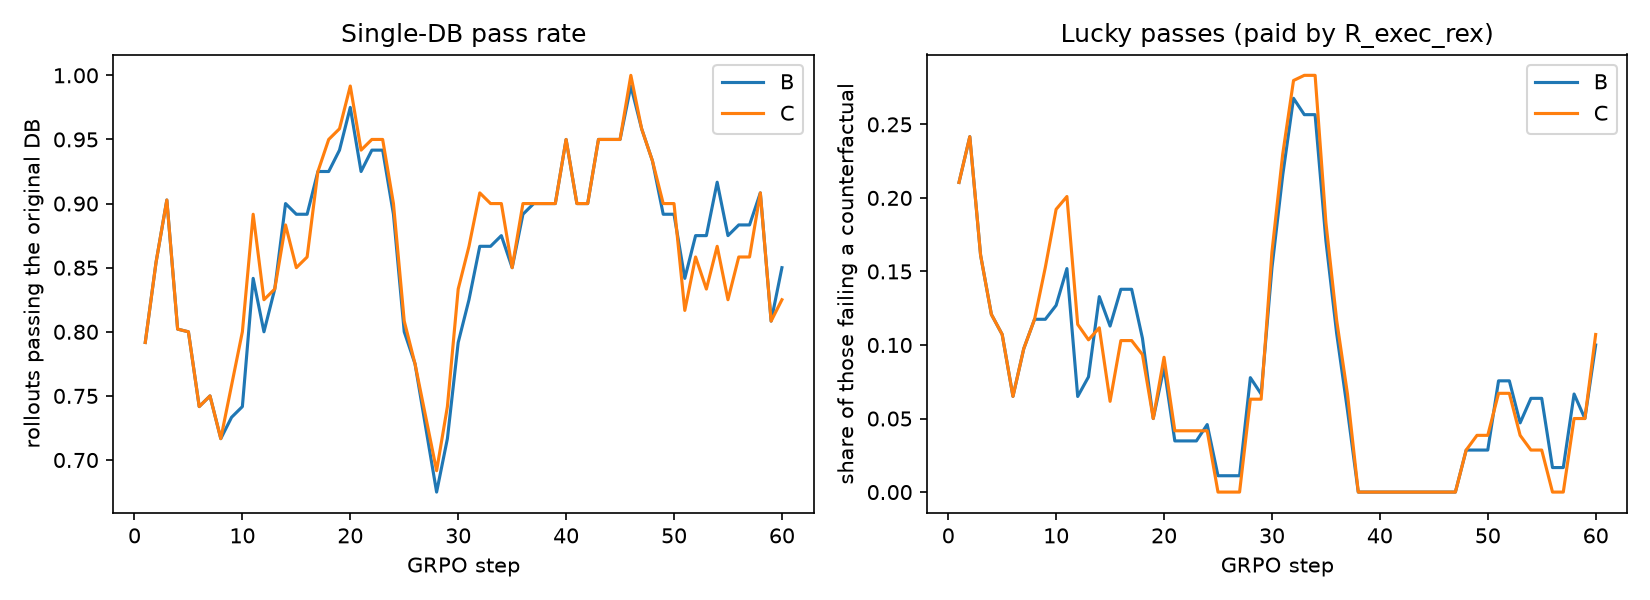
\includegraphics[width=\linewidth]{figure3_training_rewards.png}
\caption{Per GRPO step for runs B and C: share of rollouts passing the original database (left), and share of those that fail a counterfactual, i.e.\ lucky passes the single-database reward pays (right).}
\label{fig:train}
\end{figure}

\paragraph{Manual audit.} We labelled 48 wrong test trajectories by hand (16 per model, seed 0, stratified by family; 18 lucky passes) with the NL2SQL-BUGs taxonomy \citep{liu2025nl2sqlbugs}. The most common errors were \code{order\_date} used for payment date (11), product category matched against customer columns or hallucinated values (7), an extra status filter (6), a missing latest-row filter (5) and AVG over items instead of per-order totals (5). \textbf{Every lucky pass is a real semantic bug}, and none of the 48 is smuggling or reward hacking: the single-database reward's false positives on this agent are honest mistakes, exactly what counterfactual databases catch. With 16 per model, the audit cannot separate B from C.

\subsection{Why the null}
\label{sec:null}

The training comparison is null, and it is neither noise nor evidence that the counterfactual reward hurts. (1) \textbf{C really was stricter}: in replay, C's reward was lower than B's on 7.1\% (B run) and 7.2\% (C run) of rollouts, and higher on only 0.1\% and 0.3\%. (2) \textbf{The prompts were too easy for the difference to matter}: with 86\% of rollouts passing the original database, the rewards agreed on about 93\% of rollouts. Optimisation speed depends on reward variance under the policy, not on reward accuracy alone \citep{razin2025reward}, and RLVR tolerates far more reward noise than 7\% \citep{lv2025noisy}. (3) \textbf{Others see the same pattern}: DualSQL \citep{dualsql2026} trained Qwen3-8B with a stricter single-database comparator and gained +0.4 EX. Also, with all 11 train templates in SFT, the SFT model solved the GRPO prompts deterministically (only 8 of 2670 rollouts were lucky passes), so we held 3 templates out of SFT to make the rewards differ at all.

\section{Selection without gold, and cost}
\label{sec:e8}

\paragraph{Self-consistency.} Picking each item's most common answer out of 8 samples, with no gold, raises verified accuracy (Table~\ref{tab:e8}). Voting on 5 databases adds nothing over voting on 1 (within $\pm1$ pt for every model). A ``shaky answer'' flag (fewer than half the samples agree) catches 53--59\% of wrong answers at 94--98\% precision, again with no gain from the extra databases (AUROC 0.67--0.74). This is a null: at 10--15\% accuracy, wrong answers rarely agree, so one database already splits them. All three trained models reach about the same pass@8 (21.5--22.4\%), so GRPO-B's gain is in picking its right answer more often, not in finding new ones.

\begin{table}[t]
\caption{Selection without gold over 8 samples (paired bootstrap CIs over items).}
\label{tab:e8}
\centering\small
\begin{tabular}{lccccc}
\toprule
Model & First sample & Vote, 1 DB & Vote, 5 DBs & Any of 8 (oracle) & 5-DB vote $-$ first\\
\midrule
SFT & 8.5\% & 10.9\% & 11.8\% & 21.5\% & +3.3\ci{+0.6}{+6.3}\\
GRPO-B & 13.9\% & 16.9\% & 16.3\% & 22.4\% & +2.4\ci{-0.6}{+5.4}\\
GRPO-C & 6.3\% & 13.6\% & 13.9\% & 21.5\% & +7.6\ci{+4.8}{+10.6}\\
\bottomrule
\end{tabular}
\end{table}

\paragraph{ROI against a closed model.} Cohere Command A answers each test item once, single-turn, with the schema in the prompt and no tools; cost is billed tokens at list price (\$2.50 / \$10.00 per 1M input / output tokens). Tiny Aya cost is the L4 on-demand rate (\$0.74/hr) times measured generation time.

\begin{table}[t]
\caption{Cost per 1k queries and per 1k verified-correct answers.}
\label{tab:roi}
\centering\small
\begin{tabular}{lcccc}
\toprule
Model & Verified & \$ / 1k queries & \$ / 1k verified & Throughput\\
\midrule
Command A & 81.0\%\ci{76.4}{84.8} & \$4.24 & \$5.24 & median 9.7 s per query\\
Tiny Aya SFT & 9.4\%\ci{8.4}{10.6} & \$0.054 & \$0.57 & 3.8 traj/s on L4 (scaled)\\
Tiny Aya GRPO-B & 12.7\%\ci{11.5}{14.0} & \$0.061 & \$0.48 & 3.4 traj/s on L4 (measured)\\
Tiny Aya GRPO-C & 9.0\%\ci{7.9}{10.1} & \$0.052 & \$0.58 & 4.0 traj/s on L4 (scaled)\\
\bottomrule
\end{tabular}
\end{table}

The small model is about 70$\times$ cheaper per query and about 11$\times$ cheaper per verified-correct answer (Table~\ref{tab:roi}), but at 12.7\% accuracy it does not replace Command A. Command A also falls into the fan-out trap: 0\% verified on all 36 items of one F2 template, where joining \code{payments} directly double-counts orders with two payments. The single-database check rejects 32 of those 36; the counterfactual copies reject the other 4, which match on the original by luck.

\section{Related work}
\label{sec:related}

Checking SQL on more than one database is not new. \citet{pasupat2016inferring} used fictitious worlds to rule out spurious logical forms; \citet{zhong2020semantic} built distilled test suites for \emph{evaluation}, which our Spider check reuses; SpotIt \citep{klopfenstein2025spotit} searches for a distinguishing database with an SMT solver, also for evaluation; \citet{ai2026counterfactual} evaluates on counterfactual database instances; and SQLoom \citep{sqloom2026} uses counterexample databases for supervised fine-tuning. ReViSQL \citep{revisql2026} is closest: it finds that 28.8--38.4\% of positive execution rewards are refuted by VeriEQL, close to our 29.5\%, and softens the reward to 0.8 at frontier scale on one database. DualSQL \citep{dualsql2026} trains 4B/8B models with a stricter comparator and sees a near-null. Outside SQL, \citet{helff2026gaming} show RLVR opening a hacking gap against a normal verifier that a perturbation verifier closes. Gold noise is a further reason to prefer generated databases with trusted gold \citep{jin2026annotation}. Our delta is (1) code-generated copies per bug family, with no solver, used as a hard RL reward at 3B in a run where the reward is the only variable; (2) a mutant-and-hack audit of the reward itself, applied to two public rewards and eight real systems; and (3) an upstream fix for the AgentTune exploit.

\section{With more credits: a pre-registered test}
\label{sec:prereg}

The null says our prompts were too easy, not that the reward is useless. We fix the next test now.
\textbf{Curriculum:} sample SFT 8 times on small-slice (about 50-customer) train items; keep items where 1--7 of 8 samples pass the original database and at least 20\% of those passes fail a copy.
\textbf{Runs:} B ($\Rrex$) vs C-min ($\Rcf^{\mathrm{strict}}$) vs C-penalty ($-0.5$ on a lucky pass), 3 seeds each, 120 steps, everything else as in \S\ref{sec:method}, same test set.
\textbf{Prediction:} C-min beats B by at least 2 pts verified (mean of 3 seeds), and B's lucky-pass share of training rollouts rises over steps while C-min's does not. If the gap is under 2 pts, or its 3-seed CI includes 0, we report a second null.

\section{Limitations}
\label{sec:limits}

\begin{itemize}
  \item \textbf{One seed} per training condition; the B--C gap is significant across test items but not across runs.
  \item \textbf{One model} (Tiny Aya Global 3.35B) and 60 GRPO steps on one L4 GPU.
  \item \textbf{Synthetic schemas:} one e-commerce schema and 18 templates. The Spider check is the only real-data result, and it uses other systems' predictions, not our model's.
  \item \textbf{Gold-informed copies:} copies are generated from each item's bug families, which know the gold query. A deployable verifier would build them from the schema alone.
  \item \textbf{Comparator:} our strict comparator is stricter than the official Spider script, so Spider EX/TS are not leaderboard numbers. The test generator is less strict than the training reward (it catches 54 of 103 base-blind mutants).
\end{itemize}

\section*{Artifacts, models and licences}

\begin{itemize}
  \item \textbf{Lexsi repositories:} AgentTune (\code{d4db4c1}): multi-turn GRPO with tools, its render, parse and fold functions, and provenance; one trainer patch and one reward fix (\S\ref{sec:public}). AuditKIT (\code{9da5838}): silent-error framing and pass$^k$.
  \item \textbf{Models:} \code{CohereLabs/tiny-aya-global} (CC-BY-NC-4.0, gated), the trained policy. Cohere Command A (\code{command-a-03-2025}), ROI comparison only.
  \item \textbf{Adapters:} \href{https://huggingface.co/sqlcf-lexsi/tiny-aya-global-sqlcf-sft}{SFT}, \href{https://huggingface.co/sqlcf-lexsi/tiny-aya-global-sqlcf-grpo-b}{GRPO-B}, \href{https://huggingface.co/sqlcf-lexsi/tiny-aya-global-sqlcf-grpo-c}{GRPO-C}: LoRA $r$=16, each shipping the base model's licence, gated with automatic approval.
  \item \textbf{Data:} \href{https://huggingface.co/datasets/sqlcf-lexsi/counterfactual-sql-data}{\code{sqlcf-lexsi/counterfactual-sql-data}}: items, all SQLite databases, SFT trajectories, every GRPO rollout with its per-database pass vector and reward, and every test trajectory. Synthetic, CC-BY-NC-4.0.
  \item \textbf{Code:} \url{https://github.com/RishiiGamer2201/sexsi_hack}. \code{python verify\_all.py} re-derives every number in this paper from stored runs.
\end{itemize}

\begin{thebibliography}{99}\small

\bibitem[Ai(2026)]{ai2026counterfactual}
Ai.
\newblock \emph{arXiv:2608.16663}, 2026.

\bibitem[Lexsi~Labs(2026)]{agenttune2026}
Lexsi Labs.
\newblock {AgentTune}.
\newblock \emph{arXiv:2610.13335}, 2026. \url{https://github.com/Lexsi-Labs/AgentTune}.

\bibitem[Chen et~al.(2026)]{dualsql2026}
Chen et~al.
\newblock {DualSQL}.
\newblock \emph{arXiv:2609.18135}, 2026.

\bibitem[Cohere~Labs(2026)]{tinyaya2026}
Cohere Labs.
\newblock Tiny {Aya} {Global}.
\newblock \url{https://huggingface.co/CohereLabs/tiny-aya-global}, 2026.

\bibitem[Fu et~al.(2026)]{sqloom2026}
Fu et~al.
\newblock {SQLoom}.
\newblock \emph{arXiv:2611.03298}, 2026.

\bibitem[Helff et~al.(2026)]{helff2026gaming}
Helff et~al.
\newblock {LLMs} gaming verifiers: {RLVR} can lead to reward hacking.
\newblock \emph{arXiv:2604.15149}, 2026.

\bibitem[Jin et~al.(2026)]{jin2026annotation}
Jin, Choi, Zhu, and Kang.
\newblock Pervasive annotation errors break text-to-{SQL} benchmarks and leaderboards.
\newblock \emph{arXiv:2601.08778}, 2026.

\bibitem[Klopfenstein et~al.(2025)]{klopfenstein2025spotit}
Klopfenstein, He, Wang, Tremante, Wu, and Narodytska.
\newblock {SpotIt}: evaluating text-to-{SQL} evaluation with formal verification.
\newblock \emph{arXiv:2510.26840}, 2025.

\bibitem[Liu et~al.(2025)]{liu2025nl2sqlbugs}
Liu et~al.
\newblock {NL2SQL-BUGs}: a benchmark for detecting semantic errors in {NL2SQL} translation.
\newblock In \emph{KDD}, 2025. \emph{arXiv:2503.11984}.

\bibitem[Lv et~al.(2025)]{lv2025noisy}
Lv, Xie, Sun, Kang, and Yan.
\newblock The climb carves wisdom deeper than the summit: on the noisy rewards in learning to reason.
\newblock \emph{arXiv:2505.22653}, 2025.

\bibitem[Ma et~al.(2025)]{ma2025sqlr1}
Ma et~al.
\newblock {SQL-R1}: training natural language to {SQL} reasoning model by reinforcement learning.
\newblock In \emph{NeurIPS}, 2025. \emph{arXiv:2504.08600}.

\bibitem[NovaSky-AI(2025)]{skyrl2025}
NovaSky-AI.
\newblock {SkyRL-SQL}.
\newblock \url{https://github.com/NovaSky-AI/SkyRL}, 2025.

\bibitem[Pasupat and Liang(2016)]{pasupat2016inferring}
P.~Pasupat and P.~Liang.
\newblock Inferring logical forms from denotations.
\newblock In \emph{ACL}, 2016.

\bibitem[Razin et~al.(2025)]{razin2025reward}
N.~Razin et~al.
\newblock What makes a reward model a good teacher? {An} optimization perspective.
\newblock In \emph{NeurIPS}, 2025. \emph{arXiv:2503.15477}.

\bibitem[Zhu et~al.(2026)]{revisql2026}
Zhu, Jin, Choi, and Kang.
\newblock {ReViSQL}.
\newblock \emph{arXiv:2603.20004}, 2026.

\bibitem[Yao et~al.(2024)]{yao2024taubench}
S.~Yao, N.~Shinn, P.~Razavi, and K.~Narasimhan.
\newblock $\tau$-bench: a benchmark for tool-agent-user interaction in real-world domains.
\newblock \emph{arXiv:2406.12045}, 2024.

\bibitem[Yao et~al.(2025)]{yao2025arctic}
Yao et~al.
\newblock {Arctic-Text2SQL-R1}: simple rewards, strong reasoning in text-to-{SQL}.
\newblock \emph{arXiv:2505.20315}, 2025.

\bibitem[Yu et~al.(2018)]{yu2018spider}
T.~Yu et~al.
\newblock Spider: a large-scale human-labeled dataset for complex and cross-domain semantic parsing and text-to-{SQL} task.
\newblock In \emph{EMNLP}, 2018.

\bibitem[Zhong et~al.(2020)]{zhong2020semantic}
R.~Zhong, T.~Yu, and D.~Klein.
\newblock Semantic evaluation for text-to-{SQL} with distilled test suites.
\newblock In \emph{EMNLP}, 2020.

\end{thebibliography}

\end{document}
